\newpage
\subsection{The camera}
The camera is a Lumix DMC-G5. This model has been used in a similar project called micrObs to take pictures of penguins in Antarctica. In this project, the camera has successfully been retro engineered in order to control it automatically. The system to control the camera is explained in the 3.5. part.

\begin{figure}[!h]
    \centering
    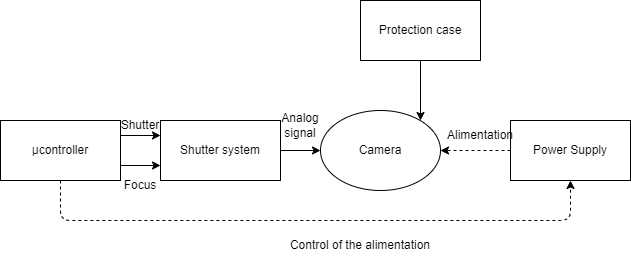
\includegraphics[width=0.9\textwidth]{\currfiledir/figures/camera_diagram.png}
    \caption{Architecture of the system surrounding the camera}
\end{figure}

The camera need a lens to be mounted on it in order to make it work properly. The calculations realized show the lens should be a lens with a focal length between 45 and 150 mm.

Here is the calculation:

\begin{figure}[!h]
    \centering
    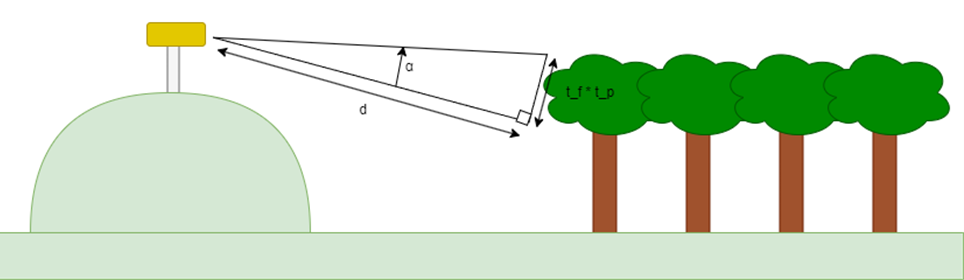
\includegraphics[width=0.85\textwidth]{\currfiledir/figures/calculation_schema.png}
    \caption{Schematic to calculate the focal length for the camera.}
\end{figure}

\noindent\(\alpha\): lens angle of the field of a (to calculate)\\
\(d\): distance between our system and trees (equal to 300 metres)\\
\(t_f\): size of a leaf, estimated to be 5,5 centimetres.\\
\(t_p\): height of the image, which corresponds to 1024 pixels.\\

\noindent According to the trigonometric formulas: \(\alpha=arctan\left(\frac{t_f*t_p}{d}\right)=32,4\textdegree\)

\newpage
%Schematic of different focal lengths
\begin{figure}[!h]
    \centering
    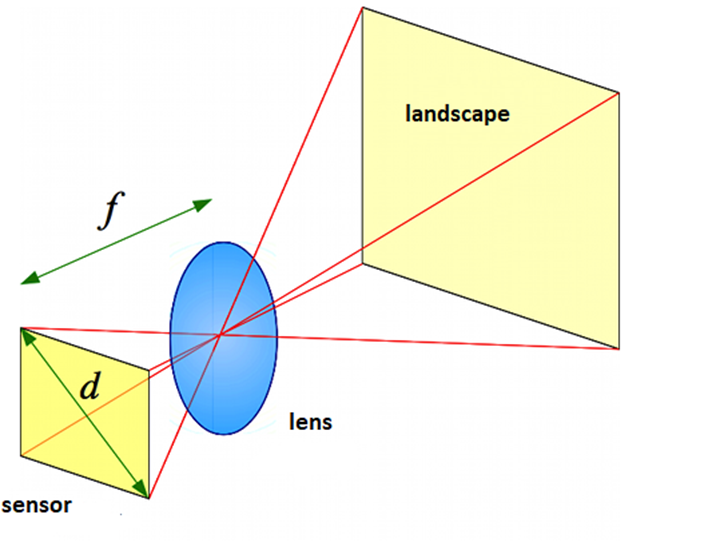
\includegraphics[width=0.75\textwidth]{\currfiledir/figures/calculation.png}
    \caption{Link between angle of view and focal length}
    \cite{focal_length}
\end{figure}

The field of view angle \((\alpha\)) horizontally, corresponding to the length (L) of the sensor, is given by the following formula:
% f=L/(2*tan⁡(α/2) )
\begin{equation}
    f=\frac{L}{2*tan\left(\frac{\alpha}{2}\right)}
\end{equation}

\noindent Where:\\
L: length of the sensor in mm\\
f: focal distance of the lens in mm\\
\(\alpha\): lens angle of the field of view\\
It is obtained: f = 117 mm\\

The equivalent focal length of a Micro 4/3 lens with a field of view of 32.4 degrees is approximately 117 mm.\\


\noindent According to the graph above, we should choose a lens between 100 and 200 mm. The smaller the angle of view (high focal length), the greater the magnification (long focal lengths will give the impression of being closer to the scene captured).\\
Our goal is not to visualize each leaf but each branch so a lens with a focal length of 175 mm will be sufficient for our project.\\
We have therefore selected this objective: \url{https://www.m43lenses.com/panasonic-45-175mm-f4-5.6/}